\documentclass[11pt,english,a4paper]{article}
\usepackage[utf8]{inputenc}
\usepackage[T1]{fontenc}
\usepackage{graphicx, url}
\usepackage[bottom]{footmisc}

\title{Parsing the Wikipedia Dumps}
\author{Ingrid Grønlie Guren}

\begin{document}

\maketitle

% url for footnotes
\urldef\nowikidump\url{http://dumps.wikimedia.org/nowiki/latest/}
\urldef\categorytree\url{http://no.wikipedia.org/w/index.php?title=Spesial%3AKategoritre&target=Astrid+Lindgren&mode=categories&namespaces= }.
\urldef\olejohandahleng\url{http://en.wikipedia.org/wiki/Ole-Johan_Dahl}


\subsection*{}
In the beginning, I have worked with the Norwegian Wikipedia Dumps \footnote{\nowikidump}, since this is the language I am most familiar with. But all the programs written should also work with dumps in other languages.  


\subsection*{Structure of Wikipedia}
Wikipedia has a structure where all articles are sorted into categories. This means that a category have articles, but could also have subcategories, where the subcategories have their own articles and subcategories. The categories form a large category tree where articles are put under the most describing category. For instanece will Ole Johan Dahl \footnote{\olejohandahleng} (Norwegian computer scientist) be placed under the category \textit{Norwegian computer scientists} instead of the parent category \textit{Computer scientists by nationality}.

Figure \ref{fig: subcat_lindgren} is an example of a structure for the category \textit{Astrid Lindgren}, a famous Swedish author of children books. The figure is an example of a the tree structure of categories. The figure shows that the category \textit{Astrid Lindgren} has 7 pages directly under the category, and 3 subcategories: \textit{Astrid Lindgrens karakterer} (7 pages), \textit{Astrid Lindgrens bøker} (9 pages) and \textit{Pippi Langstrømpe} (16 pages).  This means that there are inderictly 39 pages under the category \textit{Astrid Lindgren}. 

%is created and how it is fetched from the page for category information.\footnote{\categorytree}

\begin{figure}
\centering
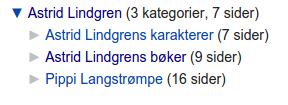
\includegraphics[height=3cm]{Dumps/imgs/Kategorier-Astrid-Lindgren.png}
\caption{Subcategories of the category \textit{Astrid Lindgren}. }
\label{fig: subcat_lindgren}
\end{figure}

An article in Wikipedia can be categorized under more than one category. This does not necessarily mean that the categories are equal, but that the article has content that can be categorized under more than one category. Some of these categories might therefore be unnecessary or redundant, where the the combination of two specialized categories might not provide more information. An example of a specialized category is the article of \textit{Ole Johan Dahl}. Some of the article's categories are showed in fiugre \ref{Fig: olejohandahl_categories}. This is an example of an article where the categories provide the same information, i.e., we already know that he was from Norway since he is in the category \textit{People from Mandal, Norway}, so it would be enough to add that he was a computer scientist instead of specifying that he was a norwegian computer scientist. 

\begin{figure}
\centering

\includegraphics[width=\textwidth]{Dumps/imgs/olejohandahl-categories.png}
\caption{Some categories from the article of Ole Johan Dahl}
\label{fig:olejohandahl_categories}
\end{figure}

Removing categories that are too specified is a way of avoiding redundancy in the categories. I have noticed that the category could be grouped into there different types of categories. The first type is the categories that are very general, for instance \textit{sport} or \textit{history}. The second type of category is the category that is only used to sort its subcategories. The category \textit{Computer scientists by nationality} is an example of the second type of  category where there are no direct articles, but only subcategories that are more describing. Such a category will therefore be less useful in our classification. We could either remove the category, but might then loose information. We could flat the category tree, where all the subcategories' articles will be moved to the parent category. The last type of categories that I have noticed is the category that is specified towards one or more articles. Some of these might not be useful, for instance if they are specified towards only one article. 

\subsection*{Extracting the category names}
I started by downloading the latest Norwegian category dump from Wikipedia. The file was a SQL-file for creating a Database with all the articles. This means that all the articles with their name was in a long \texttt{INSERT} statement. 

%For each category, a new entry was made containing a lot of the needed information and some information that where not needed for our task. 

Each category in the database entry was stored with information about the category, including the id for the category in the database (a number counting from 0), the name of the category, number of pages directly under the category and number of subcategories under the category to mention some. Each insertion to the database included more information than actually needed for our task, so I wrote a Python program for extracting the names of all the categories in the \texttt{INSERT} statement, where all the categories where matched with a regular expression, built as \texttt{'\(.*?\)'} to match all category statements on the form: 
\begin{verbatim}
(285112,'Norwegian_dance_musicians',0,0,0),
\end{verbatim}
This program, \texttt{Category\_dumps.py}, give a file containing 184 254 category names as result, where the category names are sorted alphabetically. 




%All categories, stored with:
%  - id (counting from 1) (auto-increment)
%  - name of the category
%  - pages (number of pages wihtin the category?)
%  - subcats  - subcategories
%  - cat-files : ??

\newpage




\begin{figure}
\centering

\includegraphics[width=\textwidth]{Dumps/imgs/Astrid-Lindgren-Wikipage-short.png}
\caption{Categories of the Wikipedia page "Astrid Lindgren"}
\label{fig: wikipage_lindgren}
\end{figure}

There also exists some linking between categories. \\\\

The Wikipedia page about Astrid Lindgren \ref{fig: wikipage_lindgren}\\\\

The relationship between articles and categories in Wikipedia is that \\\\

Categories also have some linking between the categories. \\\\



Hvilke kategorier linker til kategorien "Astrid Lindgren"?
\begin{itemize}
\item Anbefalte artikler
\item Artikler hvor bilde er det somme som på Wikidata
\item Artikler med fødested froskjellig fra Wikidata
\item Artikler uten comcat
\item Astrid Lindgren
\item Dødsfall i 2002
\item Forfattere av fantastisk litteratur
\item Fødsler i 1907
\item Kvinner
\item Litteris et Artibus
\item Objektivitet
\item Personner fra Vimmerby kommun
\item Svenske barnebokforfattere
\item Scenske forfattere

\end{itemize}
%(24,'Anbefalte_artikler','LINDGREN, ASTRID\nASTRID LINDGREN','2014-09-15 13:54:10','Lindgren, Astrid','uppercase','page'),(24,'Artikler_hvor_bilde_er_samme_som_på_Wikidata','LINDGREN, ASTRID\nASTRID LINDGREN','2014-09-15 13:54:10','Lindgren, Astrid','uppercase','page'),(24,'Artikler_med_fødested_forskjellig_fra_Wikidata','LINDGREN, ASTRID\nASTRID LINDGREN','2014-09-15 13:54:10','Lindgren, Astrid','uppercase','page'),(24,'Artikler_uten_comcat','LINDGREN, ASTRID\nASTRID LINDGREN','2014-09-15 13:54:10','Lindgren, Astrid','uppercase','page'),(24,'Astrid_Lindgren','LINDGREN, ASTRID\nASTRID LINDGREN','2013-03-04 08:19:29','Lindgren, Astrid','uppercase','page'),(24,'Dødsfall_i_2002','LINDGREN, ASTRID\nASTRID LINDGREN','2013-03-04 08:19:29','Lindgren, Astrid','uppercase','page'),(24,'Forfattere_av_fantastisk_litteratur','LINDGREN, ASTRID\nASTRID LINDGREN','2013-03-04 08:19:29','Lindgren, Astrid','uppercase','page'),(24,'Fødsler_i_1907','LINDGREN, ASTRID\nASTRID LINDGREN','2013-03-04 08:19:29','Lindgren, Astrid','uppercase','page'),(24,'Kvinner','LINDGREN, ASTRID\nASTRID LINDGREN','2014-09-15 13:54:10','Lindgren, Astrid','uppercase','page'),(24,'Litteris_et_Artibus','LINDGREN, ASTRID\nASTRID LINDGREN','2013-03-04 08:19:29','Lindgren, Astrid','uppercase','page'),(24,'Objektivitet','LINDGREN, ASTRID\nASTRID LINDGREN','2014-09-15 13:54:10','Lindgren, Astrid','uppercase','page'),(24,'Personer_fra_Vimmerby_kommun','LINDGREN, ASTRID\nASTRID LINDGREN','2013-03-04 08:19:29','Lindgren, Astrid','uppercase','page'),(24,'Svenske_barnebokforfattere','LINDGREN, ASTRID\nASTRID LINDGREN','2013-03-04 08:19:29','Lindgren, Astrid','uppercase','page'),(24,'Svenske_forfattere','LINDGREN, ASTRID\nASTRID LINDGREN','2013-03-04 08:19:29','Lindgren, Astrid','uppercase','page')

Har også en del underkategorier: 

The category also has some subcategories, which is categories specialized under the category topic. These are: 

Astrid Lindgrens karakterer (7 sider)

Astrid Lindgrens bøker (9 sider)

Pippi Langstrømpe (16 sider)


  




strict structure where all articles are sorted into categories. 





\end{document}